%%%%%%%%%%%%%%%%%%%%%%%%%%%%%%%%%%%%%%%%%%%%%%%%%%%%%%%%%
%%%%%%%%%%%%%%%%%%%author:rickymf4%%%%%%%%%%%%%%%%%%%%%%%
%%%%%%%%%%%%%%%%%%%%%%%%%%%%%%%%%%%%%%%%%%%%%%%%%%%%%%%%%
\chapter{实战方法}
\label{chap:11}

成功地应用深度学习技术远远不仅仅需要知道有哪些算法和这些算法的原理。一个好的机器学习实践者亦需要知道如何针对特定的应用选择算法,如何监控实验并对获得的反馈做出回应,从而优化该机器学习系统。在机器学习系统的日常开发中,实践者们需要决定是否需要搜集更多的数据,是增加还是减少模型的容量,是加上还是去掉规则化特征,是改进模型的优化,还是改进模型中的近似推理,亦或是对模型的实现程序进行调试。所有这些操作都是非常耗时的尝试,所以能够确定正确的行动方针是很重要的,而不是盲目猜测它。

这本书的大部分内容是关于各种机器学习模型、训练算法,和目标函数。这可能会造成这样的印象:成为机器学习专家最重要的本领是要了解各种机器学习技术并擅长不同类型的数学。 然而在实践中,正确地使用一个常见的算法比草率地使用一个晦涩的算法要好。算法的正确应用取决于掌握一些相当简单的方法。本章节中许多建议改编自。

我们建议如下的实际设计过程:
\begin{itemize}
\item 确定你的目标——要使用的误差度量和相应的目标价值。这些目标和误差度量应该由应用要解决的问题来驱动。
\item 尽快建立一个可以工作的端到端的工作流程,包括适当的性能指标。
\item 较好地给系统装上“仪表”来确定其性能瓶颈。诊断哪些部分的性能低于预期,以及是否是由于过度拟合、欠拟合,或数据或程序中存在着缺陷。
\item 基于来自“仪表”中特定的发现,重复地进行逐步改更,如收集新数据,调整超参或更改算法。
\end{itemize}

我们将采用街景地址号码转录系统作为一个运行的例子。 这个应用的目的是将建筑添加到谷歌地图中。街景车对建筑进行拍摄并记录照片对应的GPS坐标。通过卷积网络来识别每张照片中的地址号码,使得谷歌地图数据库可以将该地址加入到正确的位置上。关于如何开发这个商业应用程序的故事给出了如何遵循我们倡导的设计方法的一个例子。我们现在来描述这个过程中的每个步骤。

\section{性能度量}
\label{sec:11.1}
确定目标(即采用什么样误差度量)是必要的第一步,因为你的误差度量将指导你以后的所有操作。你还应该知道你想要什么级别的性能。

请记住,对于大多数应用,不可能实现绝对零误差。即使你有无限训练数据,并且可以恢复真实的概率分布,而贝叶斯误差定义了你能实现的最小错误率。这是因为你的输入特征可能不包含有关输出变量的完整信息,或者因为系统本质上可能是随机的。你也将受限于有限数量的训练数据。

由于各种原因,训练数据的量被限制了。当你的目标是构建一个一流的实际产品或服务时,你通常可以收集更多数据,但必须确定进一步减少错误率的价值,并将其与收集更多数据的成本进行权衡。数据收集可能需要时间、金钱,或给人们大带来痛苦(例如,如果你的数据收集过程涉及侵入性的医学测试)。 而当你的目标是回答在固定的基准上哪个算法的表现更好时,通常是不允许收集更多数据作为基准的训练集的。

如何给性能水平确定一个合理的期望?通常,在做学术时,我们基于以前发布的基准测试结果,可以做一些错误率的估计。而在做实际项目时,我们考虑的错误率是要让我们的应用是安全的,成本效益的,或是吸引消费者的。一旦确定了实际期望的错误率,那么为了达到此错误率将指导你的设计决策。

除了性能指标的目标值之外的另一个重要考虑是选择使用哪个指标。可以使用几种不同的性能指标来测量一个完整的包含各种机器学习组件的应用的有效性。这些性能指标通常不同于用于训练模型的损失函数。 如\secref{sec:5.1.2}所述,我们通常测量系统的准确率或错误率。

然而,许多应用需要更高级的指标。

有时一种错误的代价会比另一种更高。例如,电子邮件垃圾检测系统可能产生两种错误:错误地将合法的邮件分类为垃圾邮件,以及错误地允许垃圾邮件在收件箱中显示。

阻止合法消息比允许可疑消息通过更糟糕。 我们不是度量垃圾邮件分类器的错误率,我们可能希望用某种形式来衡量总体代价,认为阻止合法邮件的代价高于允许垃圾邮件。

有时我们想要训练一个二元分类器,用于检测一些异常事件。例如,我们将要为一个罕见的疾病设计一个医学测试。假设每百万人中只有一人患有这种疾病。我们通过简单地将分类器结果固定为无疾病,可以很容易地实现$99.9999\%$的检测精度。显然,用准确性来表征这种系统的性能的是不行的。 解决这个问题的一种方法是改为采用精度(precision)和召回(recall)的统计方法。精度是模型的检测结果中正确的比例,而召回是真实事件被模型检测到的比例。当一个检测器说没有人患这种疾病时将有完美的精度,但召回是零。当一个检测器说每个人都有疾病时将实现完全召回,但精度等于患有该疾病的人的百分比(在我们的例子中,一百万人中有一人的比例是$0.0001\%$)。当使用精度和召回时,我们通常绘制PR曲线,y轴表示精度,x轴上表示召回。当待检测的事件发生时,分类器将输出较高的分数。 例如,一个检测疾病的前馈网络的输出$\hat{y} = P(y=1\mid\Vx)$,表示医疗结果具有特征x的人的患病概率。当该输出概率分数大于某个阈值时,则认为检测到了。通过改变阈值,我们可以权衡在某召回下的精度。在许多情况下,我们希望用单个数字而不是曲线来总结分类器的性能。为此,我们将精度$p$和召回$r$转换为一个$F$分数:

\begin{equation}
        F = \frac{2pr}{p+r}.
\end{equation}

另一个方法是统计位于PR曲线下方的总面积。

在一些应用中,机器学习系统可以拒绝做决定。当机器学习算法可以估计一个决策的可信度时这是有用的,特别是如果错误的决策可能带来危害并且操作人员能够偶尔接管的话。街景转录系统就是这样一个例子。 它的任务是从照片中转录地址号码,以便将拍摄照片的位置与地图中的正确地址相关联。因为如果地图不准确,地图的价值会大大降低,所以只有在转录正确的情况下才添加地址非常重要。如果机器学习系统比人类更难获得正确的转录,那么最好的办法就是让人来替代。当然,如果机器学习系统能够大大减少运营人员必须处理的照片数量,那么它是有用的。在这种情况下使用覆盖率来作为性能指标。覆盖率是机器学习系统能产生响应的样本的比率。 可以将覆盖率和准确率进行权衡。 如果我们决绝了所有样本,则能获得$100\%$的准确率,但覆盖率减少到$0\%$。对于街景转录这个任务,目标是在保持$95\%$的覆盖率下达到人类水平的转录准确率。在这个任务上,人类水平为$98\%$。

还有可能是其它指标。 例如,我们可以衡量点击率,收集用户满意度调查等。许多专业应用领域也有应用特定的标准。

重要的是确定要先提高哪个性能指标,然后集中精力提高这个指标。没有明确的目标,很难判断机器学习系统的优化是否取得进展。


\section{默认基准模型}
\label{sec:11.2}

选择性能指标和目标后,下一步,对于任何的实际应用都是要尽快建立一个合理的端到端系统。 在本节中,我们提供了在各种情况下用哪个算法作为第一个基准方法的建议。请记住,深度学习研究进展是很快的,所以本书出版后可能会有更好的默认算法。

根据你的问题的复杂性,你甚至可能不想使用深度学习。如果你的问题可以通过正确地选择一些线性权重就能解决,你可能从一个简单统计模型开始做,如逻辑回归。

如果你知道你的问题属于“AI-完全的”类别,如物体识别,语音识别,机器翻译等等,那么你很可能通过一个恰当的深度学习模型来做出比较好的效果。

首先,根据你的数据的结构,选择一个类型的模型。如果你想做有监督学习,而且有固定大小的向量作为输入,那么使用带全连接层的前馈网络。如果已知输入的拓扑结构(例如,输入是一幅图像),那么使用卷积网络。在这些情况下,你应该从使用一些分段线性单元(ReLUs 或其推广如Leaky ReLUs,PreLus和MAXOUT)开始。如果你的输入或输出是一个序列,那么使用门控递归神经网络(LSTM或GRU)。

优化算法的合理选择是带动量的随机梯度下降法(SGD),加上带衰减的学习率(流行的衰减方法在不同的问题上表现有好有坏,包括:线性地衰减到一个固定的最小值,指数衰减,或每次遇到验证错误率趋于平稳时将学习效率降低2到10倍)。另一个非常合理的选择是Adam方法。批量归一化对优化性能有很大的影响,尤其是卷积网络和带sigmoidal 的非线性的网络。虽然你刚开始的第一个基线不用批量归一化是合理的,但如果优化似乎是有问题的,应该马上使用它。

除非你的训练集包含了数千万的例子或更多,否则你应该从开始就引入一些轻度的正规化。提前终止被普遍使用。Dropout是一种不错的正则化方法,它易于实现,并与许多模型和训练算法兼容。批量归一化也往往能降低泛化误差,而不用dropout,这是因为在用于规范化每个变量的统计估计中存在噪声。 

如果你的任务和另一个被广泛研究的任务相似的话,你可以先拷贝那些已经被证明在先前研究任务上表现最好的模型和算法,从而获得比较好的结果。你甚至可以从该任务复制一个训练好的模型。例如,一个是常见的做法是使用基于在ImageNet上训练得到的卷积网络的特征,来解决其他计算机视觉任务。

一个常见的问题是,是否要使用无监督学习,我们会在第三部分进一步介绍。这是和一些特定领域的有关的。有一些领域,如自然语言处理,都大大受益于无监督学习技术,如学习无监督词嵌入。在其他领域,如计算机视觉,目前的无监督学习技术没有优势,除了基于少量标记样本的半监督的学习。如果无监督学习对你的应用重要时,那么你可以引入它作为你第一个端到端学习的基线。否则,只有当你想解决的任务是无监督的时候,你才用无监督学习。还有,如果你发现你的初始基线过拟合了,你总是可以在后期尝试引入无监督学习。


\section{确定是否收集更多的数据}
\label{sec:11.3}

在建立了第一个端到端的系统之后,接下来便是测量我们的算法性能,并确定如何改进它。许多机器学习新手试图通过尝试许多不同的算法来进行改进。 然而,收集更多的数据往往要比改进学习算法更有效。

如何决定是否收集更多的数据? 首先,确定在训练集上的性能是否是可接受的。如果在训练集上的性能差,那么学习算法并没有利用已有的训练数据,因此没有理由收集更多数据。相反,得尝试通过添加更多的层或向每个层中添加更多隐藏单元来增加模型的大小。 此外,还得尝试改进学习算法,例如通过调整学习率等超参。如果你用的是大模型,并且对其进行了精心的调整优化,却不能很好地工作,则可能是训练数据质量的问题。数据可能含有太多噪声,或可能不包括待预测的目标输出的所需的正确输入。这时建议你从头开始,收集更干净的数据或收集更丰富的特征集合。

如果在训练集上的性能可接受,那么对测试集上的性能进行测试。如果测试集上的性能也是可接受的,那么没有什么可以做的了。如果测试集上的性能比训练集上的性能糟糕得多,那么最有效的解决方案之一便是收集更多的数据。要考虑的关键因素是收集更多数据的成本和可行性,通过其他方式降低测试集错误率的成本和可行性,以及预期能显着提高测试集性能的所需的数据量。在拥有数百万或数十亿用户的大型互联网公司,收集大型数据集是可行的,这样做的费用可能远低于其他替代方案,因此答案几乎总是收集更多的训练数据。例如,构建大规模的标记数据集是解决目标识别的最重要的因素之一。而在其他情况下,例如医疗应用,收集更多数据可能是昂贵的或不可行的。一个简单的替代收集更多数据的方法是通过调整超参(例如权重衰减系数)或通过添加正则化策略(例如dropout)来减小模型的大小或改进正则化。如果你发现即使调整正则化超参后,训练和测试性能之间的差距仍然不可接受,那么建议你收集更多的数据。

在决定要收集更多数据时,还需要决定收集多少。我们可以绘制训练集大小和泛化误差之间的关系曲线,如图\ref{fig:5_4}所示。 通过外推这样曲线,可以预测要达到某个性能水平所需要的额外训练数据量。通常,添加相对总量很小的一部分样本数量不会对泛化错误产生显着影响。因此建议你以对数标量来设置训练集的大小进行实验,例如使相邻两次实验之间的数据量加倍。

如果收集更多的数据是不可行的,唯一一个其它的方法是改进学习算法本身来改进泛化误差。这变成是一个研究领域,而不是一个单单给应用实践者一些建议的范畴。

\section{超参的选择}
\label{sec:11.4}

大多数的深度学习算法有许多超参,它们控制着算法的诸多方面。有的超参影响算法运行的时间和内存的消耗,有的则影响着模型的质量,以及在新的输入上推断出正确结果的能力。

有两种选择超参的基本方法:即人工选择和自动选择。人工选择超参需要理解超参的作用以及是如何帮助机器学习模型达到好的泛化的。自动选择超参可以大大降低对这些思想理解的需要,但它们往往有更大计算代价。


\subsection{手动超参调整}
\label{sec:11.4.1}

为了手动设置超参,你必须知道超参、训练误差、泛化误差和计算资源(内存和运行时间)之间的关系。这着这意味着建立一个坚实的基础,是在\ref{chap:5}中提到的关于学习算法有效容量的基本思想。

手动超参数搜索的目标通常是在一定的运行时间和内存的预算条件下找到最低的泛化误差。这里我们不讨论如何确定各种超参对运行时间和内存的影响,因为这是平台相关的。

手动超参数搜索的主要目的是调整模型的有效性容量来匹配任务的复杂性。 模型的有效容量受三个因素的约束:模型的表达能力,学习算法的最小化代价函数的能力,以及代价函数和训练过程使模型正则化的程度。含有更多层和每层更多隐藏单元的模型具有更高的表达能力(其能够表达更复杂的函数)。如果某些函数不能很好地最小化训练代价,或者诸如权重衰减的正则化项排除了这些函数,则训练算法不一定实际上学习所有这些函数。

泛化误差关于某个超参的关系函数绘制后通常成U形的曲线,如图\ref{fig:5_3}所示。曲线上的一个极端情况是,超参数值对应于低容量模型,使得训练误差高,而导致泛化误差高。 这是欠拟合。 另一个极端情况是,超参数值对应于高容量模型,使得训练和测试误差之间的差距大,而导致泛化误差高。 两个极端的中间的某个地方存在着最佳的模型容量,其通过结合中等大小的训练误差中和中等大小的泛化误差,来实现最低可能的泛化误差。

对于某些超参,当其值很大时会发生过拟合。其中一个例子是一层中的隐藏单元数量,因为随着隐藏单元数量的增加,模型容量会增加。而对于某些超参,当其值很小时会发生过拟合。例如,权重衰减系数的最小值0对应于学习算法的最大有效容量。

不是每个超参数都能够连续遍历整个U形曲线。许多超参数是离散的,例如一层中的单元数或maxout单元中的线性段数,因此只能沿着曲线访问几个点。有些超参是二值的。这些超参往往是一些指定是否要使用学习算法的一些可选组件的开关,比如对输入特征进行减均值和除以标准方差这些归一化的预处理步骤。这些超参数只能遍历曲线上的两个点。其他超参数则具有一些最小或最大值约束,限制它们访问曲线的某些部分。例如,权重衰减系数的最小值为零。这意味着如果模型在权重衰减值为零时欠拟合,我们不能通过修改权重衰减系数来进入过拟合区域。换句话说,一些超参数只能减掉容量。

学习率也许是最重要的超参了。如果你只有调整一个超参的时间,那么就去调整学习率。它用比其他超参更复杂的方式控制模型的有效容量(针对优化问题,学习率设置正确时,而不是特别大或特别小时,模型的有效容量达到最高)。学习率关于训练误差的是成U形曲线的,如图\ref{fig:11_1}所示。当学习率太大时,梯度下降可能无意中增加而不是减少训练误差。在理想化的二次情况下,当学习率大于等于其最优值的两倍时,就会出现这种情况。 当学习速率太小时,训练不仅更慢,而且可能永久地陷入在较高的训练误差中。我们对这种影响的理解是不足的(对于凸的损失函数这并不会发生)。

\begin{figure}[htbp] %  figure placement: here, top, bottom, or page
   \centering
   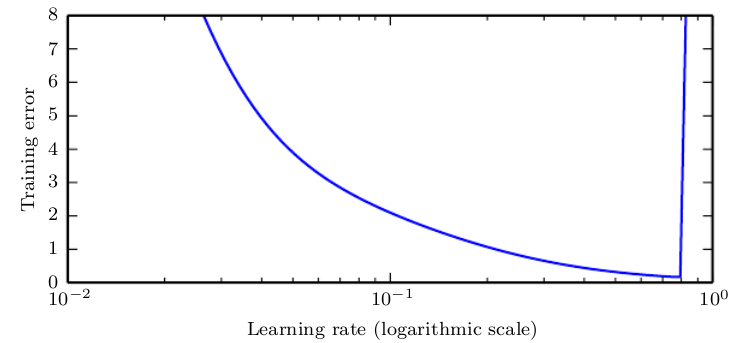
\includegraphics[width=6in]{fig/chap11/11_1.png} 
   \caption{学习率和训练误差之间的典型关系。 可以看到当学习率高于一个最佳值时误差急剧上升。这里的训练时间是固定的,因为较小的学习率有时可能仅仅减慢了训练,且减慢的速度和学习率减小量成比例。泛化误差也可以遵循该曲线,或者由于具有过大或过小的学习率而引起的正则化效应而变得复杂,因为较差的优化可以在一定程度上减少或防止过拟合,并且甚至在等效的训练误差下具有不同的泛化误差。}
   \label{fig:11_1}
\end{figure}

调整学习率以外的参数需要同时监控训练误差和测试误差,以诊断你的模型是过度拟合还是欠拟合,然后适当调整其容量。

如果你在训练集上的错误率高于你的目标错误率,除了增加模型容量没有别的选择。如果你不使用正则化,并且你确信自己的优化算法正确地执行了,则必须向网络中添加更多层或添加更多隐藏单元。但这增加了模型的计算成本。

如果你在测试集上的错误率高于目标错误率,你可以采取两种操作。测试误差是训练误差和训练与测试误差之间差距的和。通过权衡这些量可以找到最佳测试误差。神经网络通常在训练误差非常低(则容量高时)时表现得最好,并且测试误差主要由其与训练误差之间的差距来驱动。你的目标是快速地减少这个差距,而并不增加训练误差。为了减少这个差距,你要改变用于正则化的超参,以减少有效模型容量,例如添加dropout或权重衰减。最佳的性能往往来自于大模型,而且它是较好地正则化的,如使用dropout。

大多数超参可以通过推断它们是增加还是降低模型容量和设置,一些例子如表\ref{tab:11.1}所示。

\begin{table}[!hbp]
    \begin{tabular}{|c|c|c|c|}
        \hline
        \hline
        超参 & 何时可使增大容量 & 原因 & 注意点 \\
        \hline
        隐藏单元数量 & 增加 & 增加隐藏单元数量可以增加模型的表达能力 & 增加隐藏单元数量会对模型的每个操作都增加计算和内存消耗 \\
        \hline
        学习率 & 调整到最优 & 一个过大或过小的不当的学习率会导致优化失败而使得模型有效容量低 & \\
        \hline
        卷积核宽度 & 增大 & 增大卷积核宽度会增加模型的参数个数 & 较宽核的输出较窄,除非使用0填充来减小影响,否则会降低模型容量。宽核需要更多的内存来存储参数,并且计算量增加,但更窄的输出可以减少内存消耗。 \\
        \hline
        隐式0填充 & 增加 & 在卷积前加入隐式0填充可以保持较大的表达尺寸 & 对于大部分的操作都增加了时间和内容的消耗 \\
        \hline
        权重衰减系数 & 减小 & 减小权重衰减系数会让模型的参数自由而变大 &  \\
        \hline
        Dropout比例 & 减小 & Dropout单元会减少各个单元之间“合作”的机会来拟合训练集 &  \\
        \hline
        \hline
    \end{tabular}
    \caption{各种超参对模型容量的影响}
    \label{tab:11.1}
\end{table}

在手动调整超参时,不要忽视你的最终目标,即在测试集上获得良好的性能。添加正则化只是实现这一目标的一种方法。只要你具有低的训练误差,你始终可以通过收集更多的训练数据来减少泛化误差。实际中保证成功的一个暴力的方法是不断增加模型容量和训练集大小,直到任务被解决。这种方法必然增加了训练和预测的计算成本,因此只有在适当的资源下才是可行的。理论上这种方法可能由于优化困难而失败,但对于许多问题,只要选择合适的模型,优化似乎不是重要的障碍。

\subsection{自动超参优化算法}
\label{sec:11.4.2}

理想的学习算法只需要一个数据集然后输出一个函数,而不需要手动调节超参。一些比较受欢迎的算法,如逻辑回归和支持向量机源于它们本身的能力,只需调节用一、两个超参就可获得良好效果。神经网络有时可以只调节少数的超参而表现不错,但是通常需要调节四十个或更多个的超参来获得大幅度的提升。对于手动调整超参,当使用者有一个良好的起始条件,例如重用了别人的在类似的应用和架构上的初始值,或者当使用者具有类似任务的数月或多年的超参探索经验时可以获得较好的效果。然而,对于大部分应用,往往没有这样的起始条件。在这些情况下,自动算法可以找到有效的超参值。

当我们考虑一个学习算法使用者在搜索一个好的超参时所使用的方式,意识到这正是在进行优化:即我们试图找到超参的值来优化目标函数,例如验证误差,而且有时它是被一定条件约束的(例如训练耗时、内存消耗或识别耗时)。因此,理论上我们可以开发一个学习算法的选择超参的优化算法,从而将超参对使用者进行隐藏。不幸的是,超参优化算法通常有它们自己的超参,例如每个学习算法的超参应该有取值范围。然而,这些辅助超参往往更容易选择, 某种意义上,使用同样辅助超参的任务中的大部分可以获得可接受的效果。

\subsection{网格搜索}
\label{sec:11.4.3}

当存在三个或更少的超参时,通常的做法是网格搜索。对于每个超参,选择少量值的集合进行尝试。网格搜索算法然后针对超参值的集合的笛卡尔乘积后的联合值训练模型。实验后我们选择获得了最好校验误差对应的超参。如图\ref{fig:11_2}的左边,展示了一个超参值的网格。

\begin{figure}[htbp] %  figure placement: here, top, bottom, or page
   \centering
   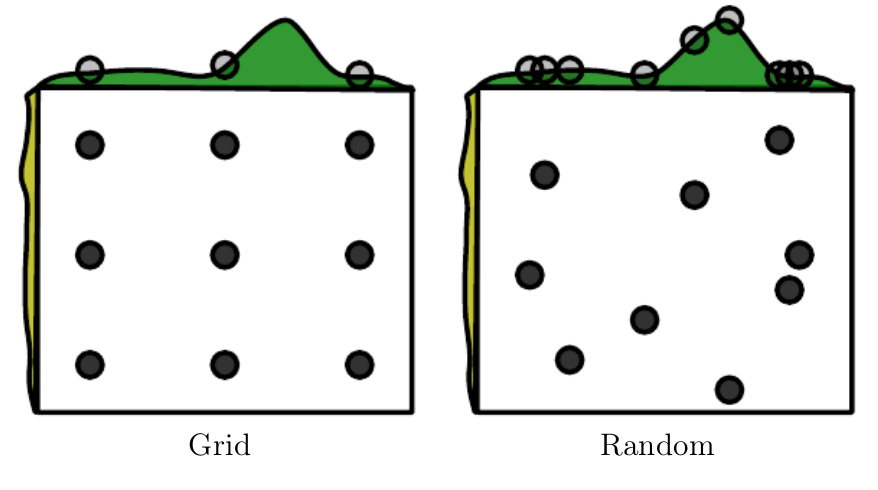
\includegraphics[width=6in]{fig/chap11/11_2.png} 
   \caption{网格搜索和随机搜索的比较。为了演示,我们展示了含有2个超参的情况,当然我们通常关注有更多超参的情况。(左)为了执行网格搜索,我们为每个超参提供一组值。搜索算法对这些集合中的每个联合超参组合运行训练。(右)为了执行随机搜索,我们提供联合超参的概率分布。通常,这些超参中的大多数彼此独立。单个超参数的常见分布包括均匀分布和对数均匀分布(对数均匀分布的采样,即从均匀分布中抽取样本进行指数运算)。搜索算法随后对联合超参组合进行随机采样,并对其中的每个组合进行训练。网格搜索和随机搜索都进行验证集错误情况的评估,并返回最佳组合。该图展示了典型情况,其中只有一些超参对结果具有显着影响。在该图中,只有水平轴上的超参具有显着的效果。网格搜索浪费了计算量,它在无影响的超参的数量上是指数级的;而随机搜索几乎在每个试验上都测试了对结果有影响的每一个超参的一个值。}
   \label{fig:11_2}
\end{figure}

应该如何选择待搜索的值列表呢?在超参是数值(有序)的情况下,根据以往在类似实验上的经验,保守地选择列表中最小和最大的值,以确保最佳值在这个范围能被选到。比较典型的是,网格搜索采用在对数尺度上近似地取值,比如在$\{0.1,0.01,10^{-3},10^{-4},10^{-5}\}$这个集合上选取学习率,或者在$\{50,100,200,500,1000,2000\}$这个集合上选取隐含单元的个数。

不断重复地执行的网络搜索往往表现得最好。比如,假设我们在超参$\alpha$的取值为$\{-1,0,1\}$上执行网格搜索。如果最佳值是1,那么我们低估了最佳$\alpha$的取值范围,进而我们应该搜索其他的取值范围,如$\{1,2,3\}$。如果我们找到的$\alpha$最佳值为0,那么我们可能希望通过放大\{-0.1,0,0.1\}来进行更加精细的网格搜索。

网格搜索的一个明显的问题是,他的计算成本随着超参的个数指数地增长。如果有$m$个超参,每个超参最多有$n$个取值,那么训练和评估试验的次数以$O(n^m)$的方式增长。试验可以平行地跑,并利用松散的并行(搜索几乎无须不同机器之间的通信)。然而,由于网格搜索的指数级的成本,即使是并行也无法提供满意的搜索规模。

\subsection{随机搜索}
\label{sec:11.4.4}

幸运的是,有一个替代网格搜索的方案,它容易编程,使用更方便,并能更快地收敛到好的超参值:随机搜索。
随机搜索按照如下步骤进行。首先我们为每个超参定义边缘分布,例如,用于二值或离散超参的伯努利分布或多项分布,或对于正实数值超参的对数均匀分布。 例如,
\begin{align}
        \texttt{log\_learning\_rate} &\sim u(-1, -5), \\
        \texttt{learning\_rate} &= 10^{\texttt{log\_learning\_rate}},
\end{align}
其中,$u(a,b)$表示区间$(a,b)$上均匀采样的样本。
同样地,$\texttt{log\_number\_of\_hidden\_units}$可从$u(\log(50), \log(2000))$上采样获得。

和网格搜索不同,我们不需要对超参进行二值化或离散化。这使得我们可以搜索更多的值而不需要增加额外的计算成本。事实上,如图\ref{fig:11_2}所示,当存在一些对性能影响不十分大的超参时,随机搜索将指数地有效于网格搜索。这在被详细地研究,他们发现随机搜索比网格搜索能更快地减少校验集误差,即每种方法更少的试验次数。
与网格搜索一样,人们往往想要运行随机搜索的多个重复版本,以基于第一次运行的结果来精细化搜索。

随机搜索能比网格搜索能更快获得好的解决方案的主要原因是它没有浪费的实验,不像网格搜索那样一个超参的两个值(给定其他超参的值)会获得相同的结果。在网格搜索的情况下,这两次运行的其他超参会具有相同的值,而对于随机搜索,它们通常具有不同的值。因此,如果这两个值的变化在校验集误差上并没有多少差别,网格搜索会不必要地重复进行两次等效实验,而随机搜索仍将给出其他超参的两次独立探索。

\subsection{基于模型的超参优化}
\label{sec:11.4.5}

可以将搜索好的超参作为一个优化问题。决策变量是这些超参。待优化的代价是用这些超参训练获得的结果在校验集上的误差。在简化的情况下,计算一些关于超参可微的校验集误差度量的梯度,我们可以简单地遵循这些梯度。然而,在大多数实际情况下,这个梯度是不可用的,因为其较高的计算和内存消耗,或由于超参本质上是在校验集误差上不可微的,比如离散值超参的情况。

了弥补这种缺乏梯度,我们可以构建一个校验集误差的模型,然后通过在这个模型下执行优化并提出一些新的超参猜测。大部分基于模型的超参搜索算法采用贝叶斯回归模型来估计每个超参的校验集误差的期望值以及期望值周围的不确定性。由此,优化需要在探索(指提出具有高度不确定性的超参,这可能导致大幅度的改进,但也可能表现不佳)和利用(指提出模型确定的超参,与目前任何超参表现一样好-通常这些超参非常类似于之前的超参)之间做权衡。当前超参优化方法包括Spearmint,TPE和SMAC。

目前我们不能明确地推荐贝叶斯超参优化法作为一个成熟工具来达到更好的深度学习结果,或者用更少的工作获得那些结果。 贝叶斯超参优化法有时表现得和人类专家相当,有时更好,但在其他问题上完败。在一个特殊问题上是值得尝试看它是否工作,但还不够成熟或可靠。那是说,超参优化是一个重要的研究领域,往往主要由深度学习驱动,而它具有贡献的潜力,不仅仅是在机器学习领域,而且是在整个工程学科。

\subsection{调试技巧}
\label{sec:11.5}

当机器学习系统表现不佳时,通常难以分辨性能不佳是算法本身固有的,还是算法实现中存在的错误。由于各种各样的原因,机器学习系统难以调试。

在大多数情况下,我们预先不知道算法的预期表现是什么。事实上,使用机器学习的整个出发点是它会的发现有用的行为,而这些是我们自己无法指定的行为。如果我们在一个新的分类任务上训练神经网络,并且它达到$5\%$的测试误差,我们没有直接的方法了解这是一个预期表现,还是一个次优的表现。

另一个困难是大多数机器学习模型具有多个部件,而且每个都是自适应的。如果一个部件坏了,其他部件仍然可以适应并达到大致可接受的性能。例如,假设我们训练具有由权重$\MW$和偏置$b$的参数的多层神经网络。其次假设我们对每个参数分别手动实现了梯度下降规则,我们做了一个错误的偏置的更新:
\begin{equation}
    \Vb \leftarrow \Vb - \alpha,
\end{equation}
其中$\alpha$是学习率。这个错误的更新没有用到梯度。这使得偏置随着训练不断地变为负数。通过检查模型的输出可能无法发现这个错误。根据输入的分布,权重可能能够适应并补偿这个负偏置。

神经网络的大多数调试策略旨在绕过这一个或这两个困难。或者我们设计一个用例可以简单地预测正确的行为,或者我们设计一个测试,单独执行神经网络的一部分。

一些重要的调试测试包括:

emph{模型执行可视化}:
当训练模型用来检测图像中的目标物体时,可以将模型的检测结果显示在图像上来观察。当训练语音的生成模型时,可以听其产生的一些语音样本。这可能看起来很明显,但是实践中很容易落入仅考虑诸如准确度或对数似然的定量性能度量。直接观察机器学习模型如何执行任务,将帮助你确定其实现的定量性能数值是否合理。对错误的评估却可能是最具破坏性的错误,因为它们可能误导你相信你系统性能是良好的,但事实上该系统性能却不好。

emph{最差样本可视化}:
大多数模型可以为所执行的任务输出某种可信度量。比如,基于softmax的分类器将一个概率值赋给每个类别。因此,分配给最可信的类所对应的概率值给出了分类器决策的置信度的估计。通常,最大似然训练导致这些值是被高估的,而不是对正确预测的一个准确概率,但它们一定程度上是有用的,因为那些实际上不大会被正确地标注的样本在模型下的概率值更小。通过查看那些对模型来说最难的训练集样本集,人们可以经常发现数据处理或标注的方法问题。比如,街景转录系统最初有一个问题,即地址号码检测系统会因将图像裁剪过小而漏掉一些数字。转录网络然后给正确答案的图像分配了将非常低的概率。由此对图像进行排序,确定了一些最可信的错误,表明裁剪出现了系统性的问题。修改检测系统以裁剪更宽的图像使得整个系统获得更好的性能,即使这会导致转录网络需要能够处理有更大变化位置和比例的地址编号。

emph{用训练和测试误差来论证软件}:
通常很难确定底层软件是否正确地实现。可以从训练和测试中获得一些线索。如果训练误差低但测试误差高,则训练过程可能是正确的,而由于基本的算法原因导致模型过拟合。另一种可能性是,训练后保存的模型被重新加载用于对测试集的评估,或者测试数据的准备与训练数据不同,这些问题导致测试误差被错误地度量。如果训练和测试误差都很高,则难以确定是否存在软件缺陷,或者是否由于基本算法原因导致模型欠拟合。这种情况需要进一步的测试,将下面描述。

emph{拟合一个小数据集}:
如果你的训练误差较大,请确定是否它是由于真正的欠拟合或由于软件缺陷。通常甚至是小模型也能保证可以拟合足够的小数据集。例如,仅通过正确地设置输出层的偏置就可以拟合具有一个样本的分类数据集。通常,如果你不能通过训练一个分类器来对单个样例进行标记,不能训练一个自动编码器来成功重现高保真的单个样例,或不能训练一个生成式模型来一直生成类似单个样例的样本,那么你的软件存在缺陷,阻碍了对训练的成功优化。这个测试可以扩展到一个只有少数几个样例的数据集上。

emph{比较反向传播的导数和数值导数}:
如果你正在使用一个需要你自己实现梯度计算的软件框架,或者如果你添加一个新的操作到求导计算库中,并必须定义它的反向传播(bprob)方法,那么常见的错误来源于梯度表达的实现错误。一个验证求导正确性的方法是比较你自己实现的自动求导所计算出的导数和有限差分计算出的导数。因为
\begin{equation}
    f'(x) = \lim_{\epsilon \to 0} \frac{f(x+\epsilon) - f(x)}{\epsilon},
\end{equation}
我们可以通过一个小的,有限的$\epsilon$来近似导数
\begin{equation}
    f'(x) \approx \frac{f(x+\epsilon) - f(x)}{\epsilon}.
\end{equation}
我们可以通过中心差分来提升近似精度:
\begin{equation}
    f'(x) \approx \frac{ f(x+\frac{1}{2}\epsilon) - f(x-\frac{1}{2}\epsilon) }{\epsilon}.
\end{equation}
扰动大小$\epsilon$必须足够大,以确保扰动不会由于有限精度的数值计算而过分舍入。
通常,我们要测试矢量值函数$g:\SetR^m \to \SetR^n$的梯度或雅可比矩阵。不幸的是,有限差分只允许我们一次求一个导数。我们既可以运行有限差分$mn$次以评估$g$的所有偏导数,又可以将测试应用于一个在$g$的输入和输出处都采用随机投影的新函数。例如,我们可以将我们的导数的实现的测试应用于$f(x) = \Vu^T g(\Vv x)$,其中$\Vu$和$\Vv$是随机向量。
正确计算$f'(x)$要求能够正确地通过$g$反向传播,但是使用有限差分来算是有效的,因为f只有单个输入和单个输出。对于有多个u和v值的情况重复这种测试通常是个不错的主意,以减少测试忽略与随机投影正交的几率。

如果可以在复数上进行数值计算,那么通过使用复数作为函数的输入能非常高效地用数值方法来估计梯度\citep{Squire+Trapp-1998}。
该方法基于如下观察
\begin{align}
    f(x + i\epsilon) &= f(x) + i\epsilon f'(x) + O(\epsilon^2) ,\\
    \text{real}( f(x+i\epsilon) ) &= f(x) + O(\epsilon^2), \quad \text{image}( \frac{f(x+i\epsilon)}{ \epsilon } ) = f'(x) + O(\epsilon^2),
\end{align}
其中$i=\sqrt{-1}$。
与上面的实值情况不同,由于取不同点处的$f$值之间的差分而没有抵消影响。这允许使用很小的$\epsilon$值,比如$\epsilon = 10^{-150}$,这使得误差对于所有实际使用的目标微不足道。

emph{监控激活和梯度的直方图}:
在大量训练迭代后(也许是一轮迭代)搜集神经网络的激活和梯度并进行统计可视化往往是非常有用的。隐藏单元的预激活值能告诉我们该单元是否饱和,或它们多久出现一次。比如,对于镇流器,他们多久关一次?是否存在某些一直关闭着的单元?对于双曲正切(tanh)单元,预激活绝对值的平均值告诉我们该单元的饱和程度。在深度网络中传播的梯度快速增长或快速消失,优化可能受到阻碍。最后,将参数梯度的幅值和参数自身的值进行比较是有用的。建议,参数在一个小批量上的更新幅度希望是参数值的$1\%$,而不是$50\%$或$0.001\%$(这会导致参数移动过慢)。也有可能是一些参数以良好的速度移动,而其它却停滞了。当数据是稀疏的(像自然语言),一些参数可能很少更新,在监控他们变化时应该记住这点。

最后,很多深度学习算法为每步产生的结果提供了一定的担保。比如,在第3节,我们会看到一些基于代数解决优化问题的近似推理算法。这些往往可以通过测试它们每个担保来调试。优化算法提供的担保包括:目标函数在算法的每步从不增长,关于某些变量子集的梯度会在算法每步变成0,以及关于所有变量的梯度会在收敛时变成0。常常,由于舍入误差,这些条件无法在数值计算中完全成立,所以调试测试应该包含一些可容忍误差的参数。

\section{示例:多位数字识别}
\label{sec:11.6}

为了端到端地描述如何应用我们的设计方法到实践中,我们从设计深度学习这个组件的角度,简单地展示下街景转录系统。显然,该系统的其他许多组件,例如街景车,数据库设施等等,也是很重要的。

从机器学习的视角出发,这个过程从数据收集开始。街景车采集了原始数据,人工操作员提供标注。转录任务开始前有大量的数据处理工作,包括使用其他机器学习技术来检测房屋号码。

转录项目开始时需要选择性能度量和相应的预期值。一个重要的总原则是使度量的选择适应该项目的业务目标。因为地图只有当它准确度高时才有用,所以为该项目设置一个高准确度的需求非常重要。具体地,以获得人类$98\%$准确度为目标。这个准确度水平可能并不总能达到。为了达到这个水平的准确度,街景转录系统牺牲了覆盖率。由此为了保持$98\%$的准确度,覆盖率变成了项目中优化的主要性能度量。随着卷积网络的改进,可以降低网络拒绝转录输入的置信度阈值,最终超出了$95\%$覆盖率的目标。

在选择量化目标后,在我们建议的方法中下一步是快速建立一个合理的基线系统。对于视觉任务而言就是一个带修正线性单元的卷积网络。转录系统从就这个模型开始。那个时候,卷积网络输出一个预测序列并不常见。为了从一个尽可能简单的基线开始,模型输出层的第一个实现由n个不同的softmax单元组成,来预测$n$个字符序列。softmax单元的训练和分类任务时的训练完全一样,每个softmax单元被单独训练。

我们推荐的方法是不断地精细化这个基线,对每个改变测试其是否带来改进。街景转录系统的第一个改变的动机来源于对覆盖率度量的理论理解和数据的结构。具体地,当输出序列的概率$p(\Vy\mid\Vx) < t$,即低于某个阈值$t$时,网络拒绝对输入$\Vx$进行分类。$p(\Vy\mid\Vx)$最初被定义为ad-hoc,即将所有softmax输出简单地相乘在一起。这促使开发一个特定输出层和代价函数,用来真正计算出合理的对数似然。这个方法使得样本拒绝机制工作得更有效。

至此,覆盖率依低于$90\%$,该方法显然没有理论问题了。因此我们的方法建议考察训练和测试集的性能,以确定问题是欠拟合或过拟合。在这种情况下,训练和测试的误差几乎是一样的。事实上,该项目进展得如此顺利的主要原因是有数以千万的标注样本可供使用。因为训练和测试误差如此相近,这表明要么欠拟合了,要么训练数据问题。我们建议的一个调试的策略是将模型最差的错误进行可视化。在这种情况下,对训练集上模型给出最高置信度的却是错误的转录进行可视化。结果显示这些大部分是由于输入图片被过度裁剪,导致一些地址的数字被删掉了。举个例子,一幅``1849''的地址图片可能被裁剪得太紧使得只有``849''可见。这个问题可以通过花费几周来提高负责确定裁剪区域的地址号码检测系统的准确性来解决。相反,这个团队采取了一个更实际的决定,即简单地扩大裁剪区域的宽度使其系统地比地址号码检测系统预测更宽。这个单一的改变使转录系统的覆盖率提高了十个百分点。

最后,性能提升的最后几个百分点来自对超参的调整。这大多数包括使模型更大同时保持一些在计算代价上的限制。因为训练和测试误差保持大致相等,所以总是清楚的是,任何性能缺陷是由于欠拟合造成的,还有一些余下的数据集本身的问题。

总之,转录系统是一个成功的项目,使得可以比人工更快速、低成本地转录数亿的地址。

我们希望本章所讲述的设计原则能引导更多其他类似的成功。

